\documentclass[xcolor=pdftex,table,11pt]{beamer}
\usetheme{Warsaw}
\usepackage[utf8]{inputenc}
\usepackage[english]{babel}
\usepackage{amsmath}
\usepackage{amsfonts}
\usepackage{amssymb}
\usepackage{multirow}
\usepackage{siunitx}
\usepackage{listings}
\usepackage{tabulary}


\usepackage[highlightcolor=yellow]{../styles/code}
\author{Informática I - Instituto Unviersitario Areonáutico}
\title{Introducción a la programación en C}

\usepackage{booktabs}
\usepackage{longtable}
\newcommand*{\thead}[1]{\multicolumn{1}{c}{\bfseries #1}}

\usepackage{tikz}
\def\checkmark{\tikz\fill[scale=0.3](0,.35) -- (.25,0) -- (1,.7) -- (.25,.15) -- cycle;} 

%\setbeamercovered{transparent} 
%\setbeamertemplate{navigation symbols}{} 
%\logo{} 
%\institute{} 
%\date{} 
%\subject{} 
\begin{document}


\begin{frame}
\titlepage
\end{frame}

\begin{frame}
\tableofcontents
\end{frame}






\begin{frame}{Estructura repetitiva while}
\begin{block}{}
 Es una estructura repetitiva controlada por centinela. Es decir, que las acciones dentro del bloque de repetición serán ejecutadas \textbf{si y sólo si} la expresión lógica evaluada en la condición de ciclo es verdadera. 
\end{block}
\end{frame}

\begin{frame}{Estructura while: pseudocódigo}

 \begin{block}{}
 Es una estructura repetitiva controlada por centinela. Es decir, que las acciones dentro del bloque de repetición serán ejecutadas \textbf{si y sólo si} la expresión lógica evaluada en la condición de ciclo es verdadera. 
\end{block}
\begin{itemize}
   \item[]<1-> Inicio del algoritmo

   \begin{itemize}
   		\item[]<2-> Mientras (condición de ciclo==Verdadera)
     	\begin{itemize}
     			\item[]<3->  acción 1;
     			\item[]<4->  acción 2;
     			\item[]<5->  acción 3;
     			\item[]<6->  ...
     			\item[]<7->  acción n;
     	\end{itemize}
   \end{itemize}
  \item[]<7-> Fin del algoritmo 
  
  
\end{itemize}



\end{frame}


\begin{frame}{Estructura while: diagrama de flujo}

 \begin{block}{}
 Es una estructura repetitiva controlada por centinela. Es decir, que las acciones dentro del bloque de repetición serán ejecutadas \textbf{si y sólo si} la expresión lógica evaluada en la condición de ciclo es verdadera. 
\end{block}
 \begin{figure}
 \centering
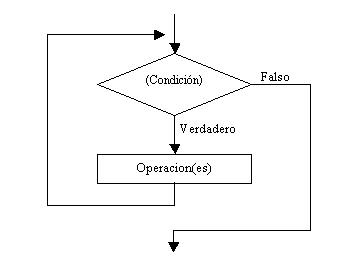
\includegraphics[scale=0.5]{../img/exported/while.jpg}
\caption{Diagrama de flujo estructura repetitiva while.}
\end{figure}
\end{frame}

\begin{frame}
\codesetstylefrombeamer
\cppfile{../../c/src/4-0-while.c}
\end{frame}




\begin{frame}{Estructura repetitiva do-while}
\begin{block}{}
La instrucción do...while es controlado por centinela pero evalúa la condición de continuación de ciclo \textbf{después de ejecutar el cuerpo del ciclo}; por lo tanto, el cuerpo del ciclo siempre se ejecutará al menos una vez.
\end{block}

\end{frame}




\begin{frame}{Estructura repetitiva do-while: pseudocódigo}
\begin{block}{}
La instrucción do...while es controlado por centinela pero evalúa la condición de continuación de ciclo \textbf{después de ejecutar el cuerpo del ciclo}; por lo tanto, el cuerpo del ciclo siempre se ejecutará al menos una vez.
\end{block}


\begin{itemize}
   \item[]<1-> Inicio del algoritmo

   \begin{itemize}
   		\item[]Hacer
     	\begin{itemize}
     			\item[]<3->  acción 1;
     			\item[]<4->  acción 2;
     			\item[]<5->  acción 3;
     			\item[]<6->  ...
     			\item[]<7->  acción n;
     	\end{itemize}
     	\item[]<8-> Mientras (condición de ciclo==Verdadera)
   \end{itemize}
   
  \item[]<9-> Fin del algoritmo 
  
  
\end{itemize}



\end{frame}



\begin{frame}{Estructura repetitiva do-while: diagrama de flujo}
\begin{block}{}
La instrucción do...while es controlado por centinela pero evalúa la condición de continuación de ciclo \textbf{después de ejecutar el cuerpo del ciclo}; por lo tanto, el cuerpo del ciclo siempre se ejecutará al menos una vez.
\end{block}


\begin{figure}
 \centering
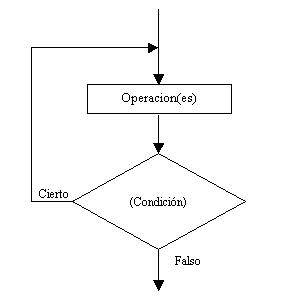
\includegraphics[scale=0.5]{../img/exported/do_while.jpg}
\caption{Diagrama de flujo estructura repetitiva do-while.}
\end{figure}

\end{frame}

\begin{frame}
\codesetstylefrombeamer
\cppfile{../../c/src/5-0-do_while.c}
\end{frame}


\begin{frame}[allowframebreaks]{Estructuras while y do-while: ejemplos}
 \begin{enumerate}
   
     \item Diseñar y codificar un programa que cuente la cantidad de números enteros ingresados por teclado. Cuando el operador ingresa el número "-1" se debe dejar de contar e imprimir el resultado.\\
\href{https://github.com/danis963/informaticaI_IUA/blob/main/c/src/4-0-while.c}{\beamergotobutton{Ver en github}}


  \item Diseñar y codificar un programa que imprima todos los números enteros comprendidos entre 0 y N. N debe ser ingresado por el operador. 
Nota: se debe usar una estructura repetitiva controlada por centinela.
\href{https://github.com/danis963/informaticaI_IUA/blob/main/c/src/4-2-while.c}{\beamergotobutton{Ver en github}}


  \item Modificar el programa anterior, para que imprima todos los números enteros comprendidos entre $N_1$ y $N_2$ ambos recibidos por teclado.
\href{https://github.com/danis963/informaticaI_IUA/blob/main/c/src/4-3-while.c}{\beamergotobutton{Ver en github}}


  \item Diseñar y codificar un programa que imprima la suma de todos los números positivos ingresados por teclado. Al ingresar un número negativo, el programa debe imprimir el valor de la suma.
\href{https://github.com/danis963/informaticaI_IUA/blob/main/c/src/5-0-do_while.c}{\beamergotobutton{Ver en github}}

  \item Diseñar y codificar un programa que permita calcular el promedio de notas de un examen parcial de un curso. El programa debe tomar notas hasta que el operador ingrese la calificación -10.
  
\href{https://github.com/danis963/informaticaI_IUA/blob/main/c/src/4-5-do_while.c}{\beamergotobutton{Ver en github}}
   \end{enumerate}
   
\end{frame}


\begin{frame}{Condiciones infinitas, sentencias break y continue}

\begin{block}{Condiciones infinitas}
Cuando en un ciclo repetitivo controlado por centinela la condición a evaluar es siempre verdadera, por ejemplo 1=1 o  2!=0, estamos en presencia de un ciclo de repetición infinito.
\end{block}

\begin{block}{Sentencia break}
Cuando una sentencia break se encuentra dentro de un bucle, este termina su ejecución y el programa continua con las líneas de código que sucedan al ciclo repetitivo.
\end{block}

\begin{block}{Sentencia continue}
Cuando una sentencia continue se encuentra dentro de un ciclo repetitivo, el programa regresa al comienzo del mismo, evitando todas las líneas que se encuentren después de haber encontrado la sentencia mencionada. 
\end{block}

\end{frame}


\begin{frame}{Sentencias break y continue: ejemplos}
 \begin{enumerate}
   
     \item Diseñar y codificar un programa que calcule la suma de 10 números ingresados por teclado. Si el operador ingresa algún número impar, el programa finalizar la toma de datos e e imprimir la suma. \\
\href{https://github.com/danis963/informaticaI_IUA/blob/main/c/src/3-4-for.c}{\beamergotobutton{Ver en github}}

   \end{enumerate}
\end{frame}

\begin{frame}{Funciones}
\end{frame}
\end{document}